%\documentclass[wcp,gray]{jmlr} % test grayscale version
\documentclass[10pt]{amsart}% former name JMLR W\&CP
%\documentclass[pmlr]{jmlr}% new name PMLR (Proceedings of Machine Learning)

 % The following packages will be automatically loaded:
 % amsmath, amssymb, natbib, graphicx, url, algorithm2e
 \usepackage{amsmath,amssymb,graphicx,url}
 \graphicspath{ {./Figures/} }
 
 \usepackage[margin=0.98in]{geometry}

 %\usepackage{rotating}% for sideways figures and tables
\usepackage{longtable}% for long tables

 % The booktabs package is used by this sample document
 % (it provides \toprule, \midrule and \bottomrule).
 % Remove the next line if you don't require it.
%\usepackage{booktabs}
\usepackage{natbib}
%\usepackage{tabularx}
 % The siunitx package is used by this sample document
 % to align numbers in a column by their decimal point.
 % Remove the next line if you don't require it.
%\usepackage[load-configurations=version-1]{siunitx} % newer version
 %\usepackage{siunitx}

% Package to make table with multi rows and columns
\usepackage{multirow}
 
 % to do
\usepackage{xcolor}
\newcommand\todo[1]{\textcolor{red}{#1}}

 % change the arguments, as appropriate, in the following:
%\jmlrvolume{}
%\jmlryear{}
%\jmlrworkshop{STA723 -- Case Study 3}
%\jmlrproceedings{}{}


\usepackage[toc,page]{appendix}


% start article
% \titlebreak
% \footnote{}
% \textsf

\title{Predictive modelling of alcohol-associated risks in college students}
 % Use \Name{Author Name} to specify the name.
 % If the surname contains spaces, enclose the surname
 % in braces, e.g. \Name{John {Smith Jones}} similarly
 % if the name has a "von" part, e.g \Name{Jane {de Winter}}.
 % If the first letter in the forenames is a diacritic
 % enclose the diacritic in braces, e.g. \Name{{\'E}louise Smith}

 % Authors with different addresses:
 
 \author{Olivier Binette \and Raphael Morsomme}
 \date{\today} % Date, can be changed to a custom date

 % Three or more authors with the same address:
 % \author{\Name{Author Name1} \Email{an1@sample.com}\\
 %  \Name{Author Name2} \Email{an2@sample.com}\\
 %  \Name{Author Name3} \Email{an3@sample.com}\\
 %  \addr Address}

 % Authors with different addresses:
 % \author{\Name{Author Name1} \Email{abc@sample.com}\\
 % \addr Address 1
 % \AND
 % \Name{Author Name2} \Email{xyz@sample.com}\\
 % \addr Address 2
 %}

% leave editor's section empty?
%\editor{Editor's name}
% \editors{List of editors' names}

\begin{document}

\maketitle

%%%%%%%%%%%%%%%%%%%%%%%%%%%%%%%%%%%%%%%%%%%%%%%%%%%%%%%%%%%%%
% INTRODUCTION
%%%%%%%%%%%%%%%%%%%%%%%%%%%%%%%%%%%%%%%%%%%%%%%%%%%%%%%%%%%%%
\section{Introduction}
\label{sec:intro}

The 2001 College Alcohol Survey is the last element of a multi-round survey carried out at three previous occasions starting in 1993. It investigated multiple aspects of student life and background information relevant to alcohol consumption and its consequences. 

Using this survey, the goal of our case study was to develop a predictive model of alcohol related risks in college students using information readily available to schools, in order to help them:
\begin{enumerate}
  \item identify students at risk and allocate support ressources as effectively as possible; and
  \item determine other pieces of information that a school might additionally gather to identify students at risk.
\end{enumerate}
To address the first question, we develop a base predictive model which takes as input a student's demographic information, information about their living accomodation on or off campus, and their GPA, in order to predict a ``ressource need'' score variable. This score variable is composed of a student awareness score and three interpretable risk scores (for consumption risks, behavioural risks, and situational risks). Responses from the College Alcohol Survey were used to score individuals in these categories and train the predictive model, and the Conformal Prediction framework \cite{Vovk.2005} is used to provide prediction uncertainty quantification.

For the second question, we studied the gain in predictive performance that can be obtained using additional predictors related to student well-being and interests. These predictors are not directly related to alcohol consumption (although one of them includes a survey question about the importance of partying) and could reasonably be probed for in order to help determine a student's level of risk. 

\subsection{Important considerations for predictive modelling}

Predictive modelling comes with particular challenges and considerations which should be addressed in the context of a real-world application. In this case study, we adress the following two points:

\begin{itemize}
\item \textbf{Meaningfulness:} We construct an interpretable and meaningful response variable that depends on (i) student awareness and (ii) three kinds of alcohol-related risks. Since we do not have the subject-matter expertise necessary to properly weight the different risks, this opens up our modelling approach to scrutiny and improvement.
\item \textbf{Reliability and out of sample performance:} We provide uncertainty quantification for the predictions with exact frequentist coverage under a data representativeness assumption. In other words, we quantify the accuracy of our model through a quantity $\Delta$ such that, for any prediction $p$, $p \pm \Delta$ is a $95\%$ confidence interval for the predicted value. This $\Delta$ is obtained through the conformal prediction framework \cite{Vovk.2005} by computing the marginal distribution of the out of sample prediction error. 
\end{itemize}

Additional issues are considered in Section \ref{sec:results}.

\subsection{Outline}

Our response variable is defined in Section \ref{sec:resp}, and our random forest predictive models are specified in Section \ref{sec:pred}. Section \ref{sec:conf} introduces the conformal prediction framework used to quantify prediction uncertainty and asssess out-of-sample predictive performance. The results of our analysis are presented in Section \ref{sec:results} and we discuss limitations and other considerations in Section \ref{sec:disc}.



\section{Materials and methods}

\subsection{Response variable}
\label{sec:resp}

We define the student ``ressource need'' variable as
$$
  \text{ressource need} = (\text{2-awareness}) (\text{consumption risk} + \text{behavioural risk} + \text{situational risk})
$$
where student awareness of alcohol risks score and other risk scores are determined from answers on the College Alcohol Survey. 

The awareness score is the complement of the mean of a school policy knowledge score (proportion of "Don't know school policy" answers to questions B3 and B5), of a school provided information score (proportion of "no provided information" on questions B6A-B6G), and of an educational material score (proportion of "no educational material or programs" on questions B7A-B7E). Figure \ref{fig:resp} shows the distribution of the constructed response variable.

For the alcohol-related risks, we looked at individual survey questions and associated to each possible answer a number between $0$ and $1$. Each of these numbers represents the marginal probability that a student providing this answer has alcohol-related issues. While it is not obvious how to aggregate these marginal probabilities without specifying a covariance structure between the questions, we opted for the complement of the geometric average of the complementary probabilities. That is, if the marginal probabilities are $p_1, \dots, p_k$, then the resulting score is $1-\prod_i (1-p_i)^{1/k}$. Missing values were omitted. In this way, having large marginal probabilities of alcohol issues on a few questions is given more weight than a low probability of alcohol issue on many questions, reflecting the fact that alcoholism can be caused by a single (or a few) factor alone. 

The consumption risk score involves the binge drinking indicator, the frequent binge drinking indicator, as well as question C7 (self-description of alcohol consumption). The behavioural risk score involves the drunk driving indicator, the binge drunk driving indicator, as well as questions C17A-C17K and questions C18E, C18F (consequences of drinking). Finally, the situational risk involves questions D1A-D1C and D1H (consequences of drinking of other students).

The measure was constructed for illustration purposes and should be refined using expert knowledge. Ideally, a model relating the different risks to the survey answers would be specified and trained using examples analyzed by experts.

\subsection{Predictive models}
\label{sec:pred}

Since we do not expect the relationship between the predictors and the response to be linear, we opt for a flexible predictive model. We choose the random forest algorithm because it offers good predictive power and requires little tuning . Due to the size of the data, a random forest takes $30$ minutes to fit, thereby limiting the possibility for tuning the parameter and conducting a sensitivity analysis. The parameters are $n=1,500$ trees, $m=p/3$ predictors considered at each split (where $p$ is the number of predictors, standard practice for regression) and the minimum number of observation per leaf is $5$.

To answer the main question of whether or not schools should collect more data about their student than what is already readily available to them in order to identify students at risk, we fit two random forest models. The \textit{baseline} model only takes for input demographic information about students (questions A1-A3, G1-G4), information about living accomodations (questions A6, A7, B9) and other information that is readily available to schools such as participation in greek life and GPA (questions A4, A5, F5, B2, B9). The \textit{augmented data} model also incorporates information about students preferences (question A8A-A8I), student activities (question F6A-F6I) and student satisfaction with life and education (questions F1-F4). Predictors with more than $25\%$ missing values were removed from the analysis and we then proceeded with a complete case analysis.

We then construct prediction intervals using the conformal prediction framework and compare their average width across the two models at various significance level. If the additional set of predictors does help make more accurate predictions, then the prediction intervals of the augmented data model will be tighter, that is, more informative.

\subsection{Conformal Prediction}
\label{sec:conf}

Conformal prediction is a framework conceptualized by Vapnik, Gammermand an Vovk in the late 90's to complement point predictions with a measure of certainty that enjoys certain properties. In the regression settings, this takes the form of prediction intervals. These prediction intervals enjoy the following properties. First, they are valid in the frequentist sense for a finite sample size, meaning that they cover the true response of the observation $\epsilon \%$ of the time, where $\epsilon$ is a set significance level, and that this property is not asymptotic. Second, the framework is distribution-free and universal. The latter qualification means that the framework can be applied to any predictive algorithm that outputs a point estimate (e.g. ridge regression, neural network, $k$-nearest neighbor algorithm or random forest to name a few). Third, these intervals can also be individualized to each observation, that is, an observation that is easy to predict will have a tight interval while an observation that is difficult to predict will have a wider interval \cite{Papadopoulos.2011}. Finally, using \textit{inductive} conformal prediction, the construction of the intervals is computationally cheap, only requiring fitting the predictive model once. This is in contrast to the bootstrap approach to the construction of prediction intervals which requires numerous fittings of the predictive models. In our case, since the random forest takes $30$ minutes to fit, bootstrap was not an option. It is worth noting that the only assumption made to construct conformal prediction intervals is the exchangeability of the observations.

We use the \textit{inductive conformal framework} \cite{Papadopoulos.2002} to construct predictive intervals. The method proceeds as follows. Given a labeled training set $\{z_i = (x_i, y_i)\}_{i=1}^n$ and an unlabeled test observation $x_{n+1}$,
\begin{enumerate}
	\item partition the training set into a \textit{proper training} set $\{z_j\}_{j=1}^l$ and a \textit{calibration} set $\{z_k \}_{k=l+1}^n$,
	\item fit the predictive model $m$ on the proper training set,
	\item compute the predictions $\hat{y}_k$ on the calibration set and the anomaly scores
	$$a(z_k, m) = |\hat{y}_k - y_k|, \quad k = l+1, \dots, n,$$
	\item identify $a_\epsilon$, the $\epsilon^{\text{th}}$ percentile of the $\{a\}_{k=l+1}^n$,
	\item compute the prediction $\hat{y}_{n+1}$ on the test observation and set the prediction interval to be
	$$\{y: |\hat{y}_{n+1} - y| < a_\epsilon\}.$$
\end{enumerate}
Note that these intervals will be the same for every observation (not individualized). In order to obtain individualized, one could use the anomaly function
$$a(z_k, m_0, m_1) = \dfrac{|\hat{y}_k - y_k|}{exp(\sigma_k)}$$
where $\hat{y}_k$ is the prediction of the response variable made the predictive model $m_0$ and $\sigma_k$ is the prediction of the log absolute error $log(|\hat{y}_k - y_k|)$ made by a second predictive model $m_1$ trained on the proper training set set. The log-exponentiation trick ensures that the anomaly values $a(z_k, m_0, m_1)$ are positive.

We use the following set-up: the test set consists of $10\%$ of the data set, the calibration set consists of $30\%$ of the training set and we repeat the procedure $10$ times to obtain the expected width of the prediction
intervals for each model at four different significance levels ($0.5, 0.75, 0.9$ and $0.95$).


\section{Results}
\label{sec:results}

Table 1 indicates that, given a significance level, the conformal prediction intervals are valid in the frequentist sense up to statistical fluctuations. Figure \ref{fig:conformal} shows the distribution of the prediction intervals. We observe that the model with the larger set of predictors produces intervals are tighter than those of the base model. Tables 2 and 3 present the $10$ variables that have the highest contribution in each model. The base predictors appears to be important predictor in the augmented model, and the \textit{parties} variables is the additional variable that has the most importance in the augmented model. 

\section{Discussion}
\label{sec:disc}

It seems that only the student's attitude towards parties seems to be complementing the variables of the base model. In fact, among the $5$ most important variables of the augmented model, it is the only one that is not present in the base model. Interestingly, it is also the most important variable of the augmented model by a large margin, indicating that collecting this variable will help schools identify more efficiently students that are at risk.

Future work should also consider the following issues relevant to the use of a predictive model. First, the use of age, race, gender, religion and other variables as predictors may be  problematic for schools. Evaluating the fairness of the model and avoiding systemic harms woulud be necessary before any potential use. Mondrian conformal prediction \cite{Vovk.2005} generates prediction intervals that are valid conditioned on the value of a given predictor (say, gender) and can therefore be used to make the model fairer. Second, we do not expect data from the 2001 College Alcohol survey to be representative of any given college in 2020. Even assuming that the alcohol risks and awareness landscape has not changed in 20 years, post-stratification or additional surveys would be necessary to properly characterize uncertainty at a given college.

\bibliographystyle{chicago}
\bibliography{bibliography}


\newpage
\appendix

\section{Figures}

\begin{center}
\begin{figure}[h]
  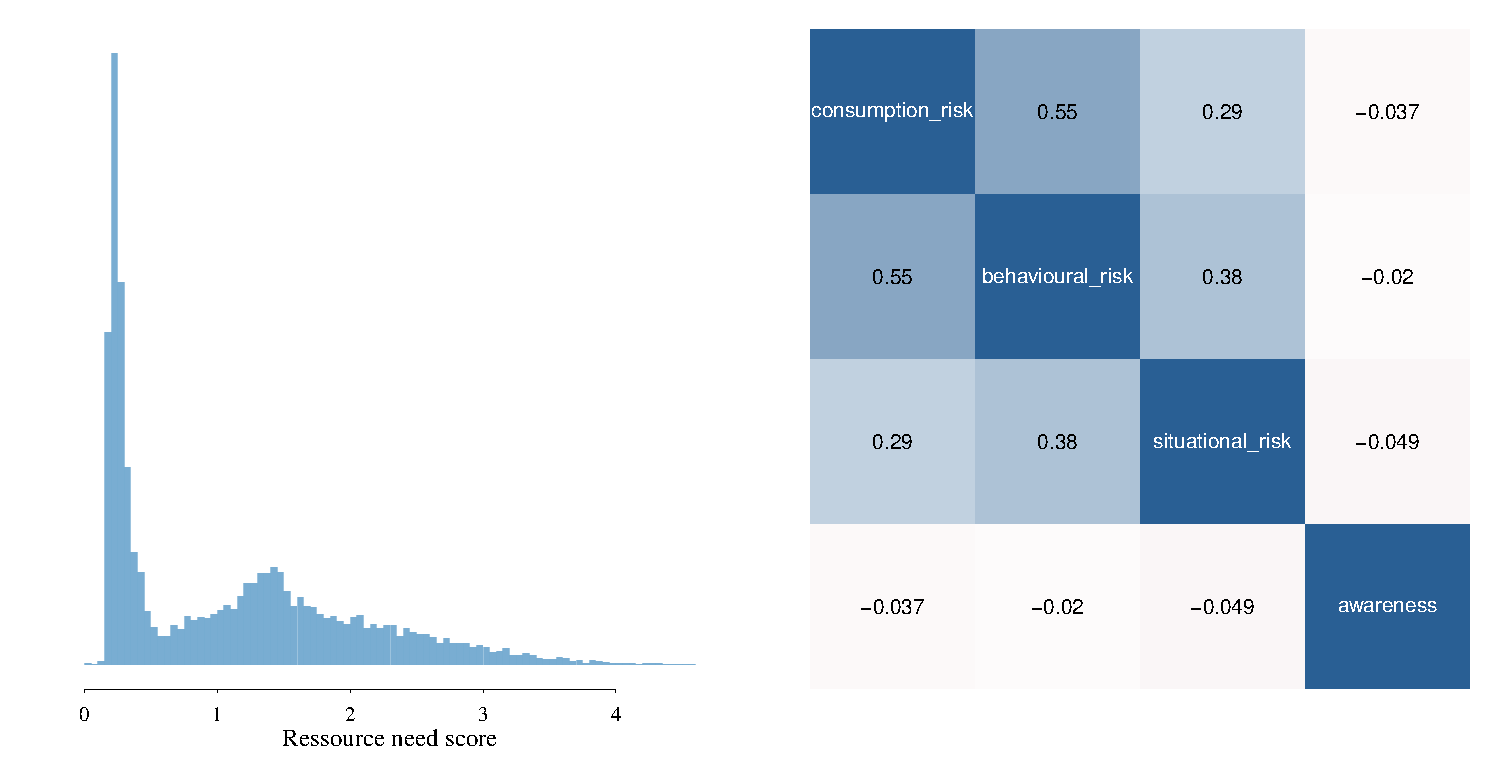
\includegraphics[width=\linewidth]{Figures/response.pdf}
  \caption{Histogram of the ``ressource need'' response variable (left) and representation of the correlation between the different components of this variable (right).}
  \label{fig:resp}
\end{figure}
\end{center}

\begin{center}
\begin{figure}[h]
  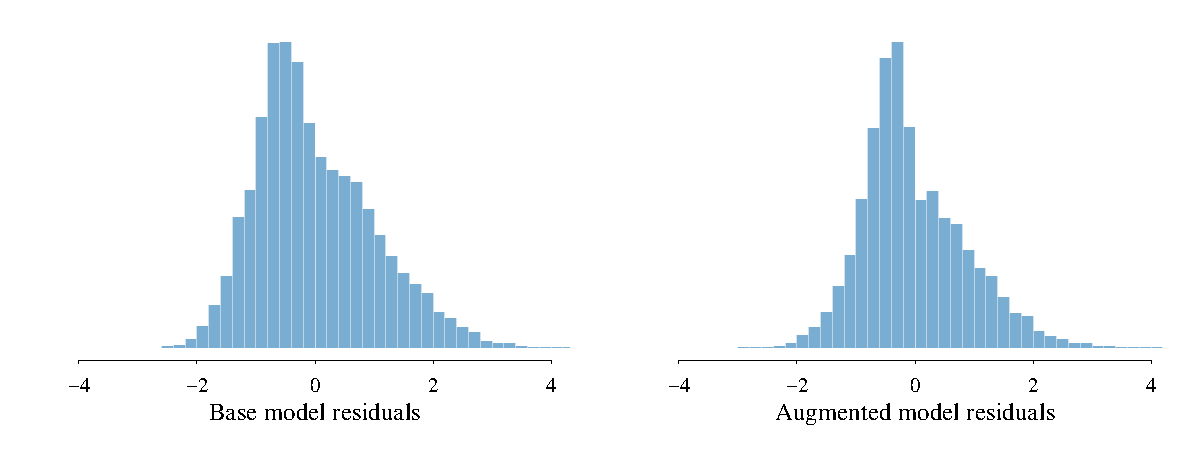
\includegraphics[width=\linewidth]{Figures/residuals}
  \caption{Histograms of predictive models residual distributions.}
\end{figure}
\end{center}


% latex table generated in R 3.5.2 by xtable 1.8-3 package
% Mon Feb 17 15:58:32 2020
\begin{table}[ht]
\centering
\begin{tabular}{rrlrr}
  \toprule
 & Significance & Set of Predictors & Mean Width & Coverage \\ 
  \midrule
1 & 0.500 & Extensive & 1.138 & 0.503 \\ 
  2 & 0.500 & Restricted & 1.370 & 0.501 \\ 
  3 & 0.750 & Extensive & 1.807 & 0.754 \\ 
  4 & 0.750 & Restricted & 2.109 & 0.749 \\ 
  5 & 0.900 & Extensive & 2.513 & 0.909 \\ 
  6 & 0.900 & Restricted & 2.801 & 0.897 \\ 
  7 & 0.950 & Extensive & 2.896 & 0.954 \\ 
  8 & 0.950 & Restricted & 3.212 & 0.951 \\ 
   \bottomrule
\end{tabular}
\caption{Coverage and Mean Width of Prediction Intervals} 
\end{table}


\begin{figure}[htbp]
	\centering
	\caption{Median and inter-decile of the width distribution of the prediction intervals across different significance levels for the two models.}
	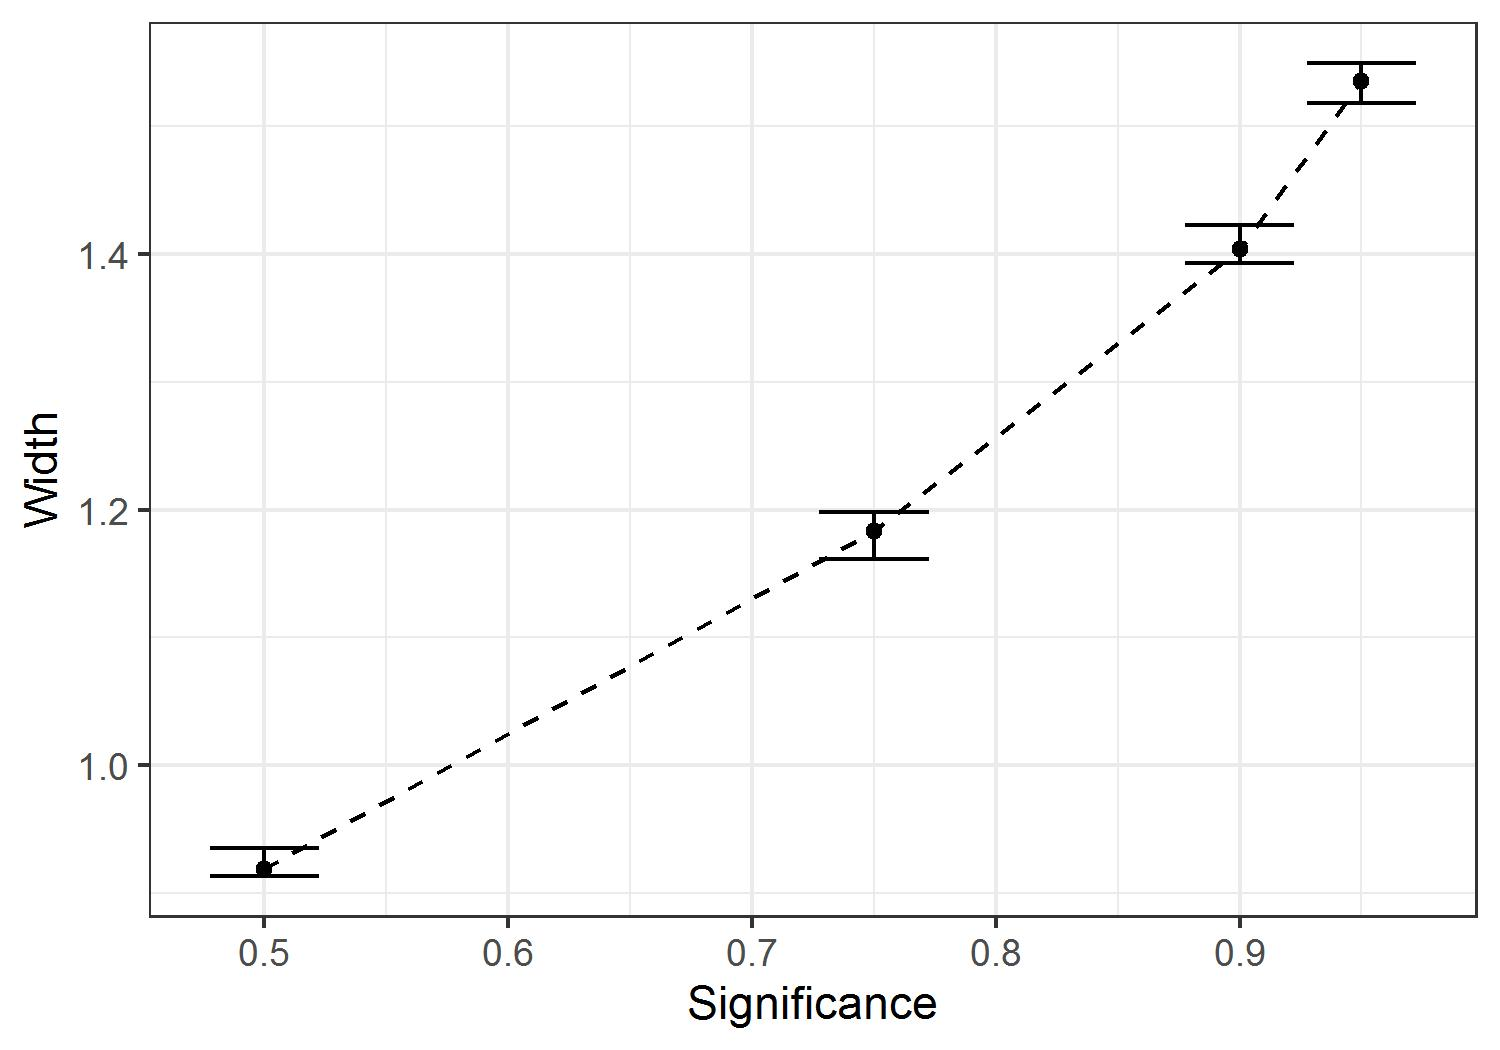
\includegraphics[width=0.9\linewidth]{conformal.jpeg}
	\label{fig:conformal}
\end{figure}

% latex table generated in R 3.5.2 by xtable 1.8-3 package
% Mon Feb 17 17:52:31 2020
\begin{table}[ht]
\centering
\begin{tabular}{rlr}
  \hline
 & Variables & Importance \\ 
  \hline
1 & race & 123.5 \\ 
  2 & roommates & 91.2 \\ 
  3 & greek\_life & 90.2 \\ 
  4 & marital\_status & 72.4 \\ 
  5 & religion & 67.6 \\ 
  6 & age & 67.1 \\ 
  7 & location & 65.1 \\ 
  8 & live\_parents & 64.9 \\ 
  9 & hispanic & 42.9 \\ 
  10 & transfer & 38.9 \\ 
   \hline
\end{tabular}
\caption{Variable importance for predictive model with restricted set of predictors} 
\end{table}


% latex table generated in R 3.5.2 by xtable 1.8-3 package
% Mon Feb 17 17:52:37 2020
\begin{table}[ht]
\centering
\begin{tabular}{rlr}
  \hline
 & Variables & Importance \\ 
  \hline
1 & parties & 268.0 \\ 
  2 & religion & 77.0 \\ 
  3 & race & 72.2 \\ 
  4 & roommates & 62.1 \\ 
  5 & greek\_life & 46.4 \\ 
  6 & marital\_status & 40.9 \\ 
  7 & socialize & 40.3 \\ 
  8 & live\_parents & 38.5 \\ 
  9 & friends & 29.3 \\ 
  10 & location & 28.1 \\ 
   \hline
\end{tabular}
\caption{Variable importance for predictive model with extensive set of predictors} 
\end{table}



\end{document}